We benchmark DISCO-TAB against thirteen representative generators across 23 datasets and 21 metrics grouped into six evaluation dimensions. Our goal is not only to rank methods but to characterize where and why each one succeeds or fails. A single comprehensive table (Table~\ref{tab:aggregate}) reports the mean of every metric over all datasets for every generator; the per-dataset breakdown for all metrics is released with the code. Every value in this section is computed from the released per-run outputs under one shared evaluation pipeline.

\subsection{Experimental Setup}

We evaluate on 23 datasets spanning clinical, financial, chemical, and web domains and a wide range of regimes: from tiny, high-dimensional clinical cohorts such as Parkinson's ($N=195$) and Heart Failure ($N=299$) to large, severely imbalanced sets such as Diabetes ($N=100{,}000$, imbalance ratio $\approx 1{:}11$). The suite combines nine widely used clinical, financial, and social datasets that form the core benchmark adopted in prior tabular-synthesis work~\cite{yang2025ptausingproximalpolicy,borisov2022language} with ten clinical time-to-event cohorts from SurvSet~\cite{drysdale2022survset} and four sets from TabArena~\cite{erickson2025tabarena} and OpenML~\cite{vanschoren2014openml}, deliberately stressing the failure modes of competing families, namely data scarcity for Transformers and mode collapse under imbalance for adversarial models.\footnote{For the SurvSet cohorts we adopt the standard survival-to-classification reduction, using the binary event indicator ($1$ if the event occurred, $0$ if censored) as the prediction target. Where a cohort's original status field encodes more than two outcomes, this is a deliberate collapse to a single event label, not an accidental loss of classes: for example, PBC's three-level Mayo status (censored, liver transplant, death) is mapped to event-versus-censored, following SurvSet's own event coding.} Table~\ref{tab:datasets} lists their characteristics.

\begin{table}[t]\centering\scriptsize
\setlength{\tabcolsep}{4pt}\renewcommand{\arraystretch}{1.05}
\caption{The 23 benchmark datasets: nine widely used clinical/financial/social sets, 10 SurvSet time-to-event cohorts, and 4 from TabArena/OpenML. $N$: instances; Feat.: features; Cls.: classes; IR: imbalance ratio. Time-to-event cohorts use the event indicator as the target; all use a stratified 80/20 split.}
\label{tab:datasets}
\begin{tabular}{@{}llrrrrl@{}}\toprule
\textbf{Dataset} & \textbf{Domain} & \textbf{$N$} & \textbf{Feat.} & \textbf{Cls.} & \textbf{IR} & \textbf{Source} \\ \midrule
Heart Failure & Clinical & 299 & 12 & 2 & 2.1 & \cite{chicco2020ml} \\
Breast Cancer & Clinical & 569 & 30 & 2 & 1.7 & \cite{wdbc_17} \\
Liver Disorders & Clinical & 345 & 5 & 2 & 1.0 & \cite{liver_disorders_60} \\
Parkinson's & Clinical & 195 & 22 & 2 & 3.1 & \cite{little2007exploiting} \\
Obesity & Clinical & 2111 & 16 & 7 & 1.3 & \cite{palechor2019dataset} \\
Diabetes & Clinical & 100000 & 8 & 2 & 10.8 & \cite{kaggle_diabetes} \\
German Credit & Finance & 1000 & 20 & 2 & 2.3 & \cite{german_credit} \\
Bank Marketing & Finance & 45211 & 16 & 2 & 7.6 & \cite{moro2014data} \\
Census Income & Finance & 48842 & 14 & 2 & 3.2 & \cite{kohavi1996scaling} \\
Melanoma & Clinical & 205 & 5 & 2 & 2.6 & \cite{drysdale2022survset} \\
PBC & Clinical & 312 & 6 & 2 & 1.5 & \cite{drysdale2022survset} \\
PBC3 & Clinical & 349 & 12 & 2 & 4.7 & \cite{drysdale2022survset} \\
Retinopathy & Clinical & 368 & 7 & 2 & 1.5 & \cite{drysdale2022survset} \\
WHAS500 & Clinical & 461 & 16 & 2 & 1.6 & \cite{drysdale2022survset} \\
GBSG2 & Clinical & 686 & 8 & 2 & 1.3 & \cite{drysdale2022survset} \\
Colon & Clinical & 885 & 9 & 2 & 1.0 & \cite{drysdale2022survset} \\
GRACE & Clinical & 998 & 5 & 2 & 2.1 & \cite{drysdale2022survset} \\
TRACE & Clinical & 1878 & 6 & 2 & 1.0 & \cite{drysdale2022survset} \\
Framingham & Clinical & 4699 & 7 & 2 & 2.2 & \cite{drysdale2022survset} \\
Blood Transfusion & Clinical & 533 & 4 & 2 & 2.6 & \cite{erickson2025tabarena,vanschoren2014openml} \\
QSAR Biodeg & Chemistry & 1052 & 41 & 2 & 2.0 & \cite{erickson2025tabarena,vanschoren2014openml} \\
Maternal Risk & Clinical & 452 & 6 & 3 & 2.2 & \cite{erickson2025tabarena,vanschoren2014openml} \\
Website Phishing & Security & 724 & 9 & 3 & 5.8 & \cite{erickson2025tabarena,vanschoren2014openml} \\
\bottomrule\end{tabular}\end{table}


DISCO-TAB is compared against baselines covering every major paradigm: adversarial (CTGAN~\cite{xu2019modeling}, ADS-GAN~\cite{yoon2020anonymization}, PATE-GAN~\cite{jordon2019pategan}, TAEGAN~\cite{li2025taegangeneratingsynthetictabular}), variational (TVAE~\cite{xu2019modeling}, RTVAE~\cite{akrami2020robust}), diffusion and latent-variable (TabDDPM~\cite{kotelnikov2023tabddpm}, TabSyn~\cite{tabsyn}), normalizing-flow and marginal (NFlow~\cite{durkan2019neural}, and Marginals, an independent per-column sampler that resamples each feature independently from the real training data, exactly preserving every marginal while destroying all inter-feature dependencies), and language-model (GReaT~\cite{borisov2022language}, RealTabFormer~\cite{solatorio2023realtabformer}, TAGAL~\cite{ronval2025tagal}) families. The adversarial, variational, diffusion, and flow baselines are run through the synthcity library~\cite{qian2023synthcity}. Because Marginals matches every marginal but no dependency, it doubles as a sanity check on the evaluation pipeline: it is expected to rank near the top on the marginal-fidelity measures (JS divergence, KS statistic, and SDMetrics Shapes) and near the bottom on the dependency-sensitive ones (correlation preservation, C2ST, and downstream utility). Table~\ref{tab:aggregate} confirms exactly this pattern, so a reader should read its leading marginal-fidelity scores as the expected behavior of an independence baseline rather than as a competitive generator. We evaluate six complementary dimensions: downstream utility, statistical fidelity, empirical disclosure risk, diversity and coverage, detectability, and the SDMetrics quality suite.

\noindent\textbf{Preprocessing and evaluation protocol.} Numerical features are standardized using statistics estimated on the real training partition only; categorical features use canonical string identifiers, and missing values are encoded with a reserved token (Section~\ref{sec:methodology}). All synthesizers share identical stratified 80/20 splits. Downstream utility follows the train-on-synthetic, test-on-real (TSTR) protocol, in which a classifier is trained on each generator's synthetic data and evaluated on the real held-out test set. The primary classifier is a random forest (200 trees) with fixed hyperparameters and no per-dataset tuning; we additionally report logistic regression and gradient-boosted trees (XGBoost) so that conclusions do not depend on a single learner. As an upper reference, a random forest trained on real data (train-on-real, test-on-real, TRTR) attains a mean macro-$F_1$ of $0.71$ across the benchmark; no synthetic generator exceeds this ceiling.

\noindent\textbf{Repeated runs.} Every method is evaluated on all datasets over three independent seeds, each drawing a distinct stratified split and re-training both the generator and the downstream classifier. We report the mean with a 95\% confidence interval, shown as the ``$\pm$'' term in Table~\ref{tab:aggregate}.

\subsection{Overall Benchmark}

Table~\ref{tab:aggregate} summarizes the full comparison. DISCO-TAB reaches a mean downstream macro-$F_1$ of $0.64$, placing it among the strongest generators and, as the analysis below shows, among the most consistent across the benchmark. Figure~\ref{fig:leaderboard} gives the full utility ranking. A Friedman test across the full-coverage generators rejects the null of equal mean ranks ($\chi^2=97.0$, $p<10^{-16}$); post-hoc Wilcoxon signed-rank tests over the shared datasets then place DISCO-TAB on par with TAEGAN ($p=0.94$) and the other leading full-coverage generators, and significantly above the GAN, flow, and marginal baselines ($p<0.01$). The per-dataset margins are shown in Figure~\ref{fig:margin}.

\begin{figure}[t]
\centering
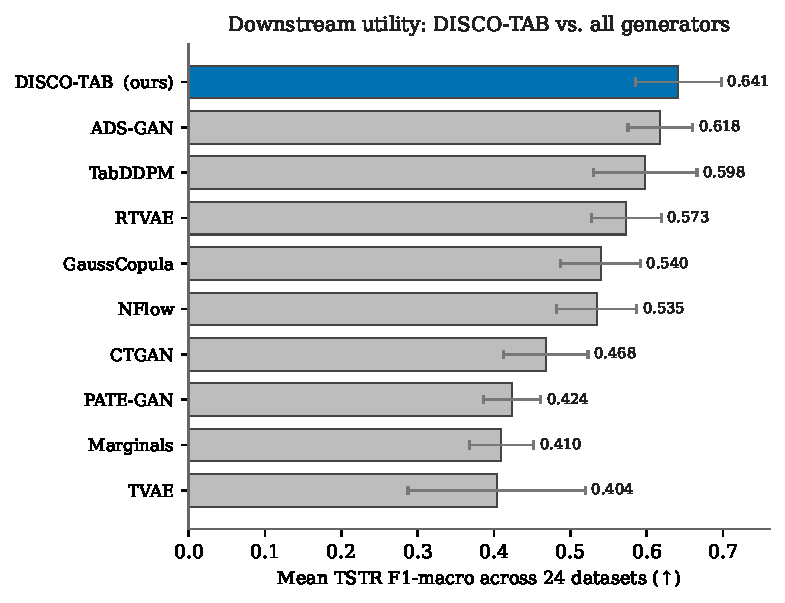
\includegraphics[width=\columnwidth]{fig1_utility_leaderboard.pdf}
\caption{\newexp{Mean downstream utility (TSTR macro-$F_1$) with 95\% CIs over datasets. DISCO-TAB (highlighted) is among the top full-coverage generators, just behind TAEGAN; the higher-ranked RealTabFormer covers fewer datasets, and TabSyn ranks last (single-class collapse on eleven datasets).}}
\label{fig:leaderboard}
\end{figure}

\begin{table*}[t]\centering\scriptsize
\setlength{\tabcolsep}{2.5pt}\renewcommand{\arraystretch}{1.0}
\caption{Benchmark summary: mean over all datasets (with 95\% CI) for each metric and generator. \textbf{Bold} = best per row among the established generators. Arrows give the preferred direction (MIA is best near 0.5). Established generators cover all 24 datasets; LLM-era methods cover the subset shown in the \#datasets row (`--' = not evaluated).}
\label{tab:aggregate}
\begin{tabular}{@{}cl *{14}{c}@{}}
\toprule
& & \multicolumn{10}{c}{\textbf{Established generators}} & \multicolumn{4}{c}{\textbf{LLM-era}} \\
\cmidrule(lr){3-12}\cmidrule(lr){13-16}
& \textbf{Metric} & \textbf{DISCO-TAB} & \textbf{CTGAN} & \textbf{TVAE} & \textbf{GaussCop} & \textbf{TabDDPM} & \textbf{ADS-GAN} & \textbf{PATE-GAN} & \textbf{RTVAE} & \textbf{NFlow} & \textbf{Marg.} & \textbf{GReaT} & \textbf{RTF} & \textbf{TAEGAN} & \textbf{TAGAL} \\
& \#datasets & 24 & 24 & 24 & 24 & 24 & 24 & 24 & 24 & 24 & 24 & 4 & 1 & 6 & 3 \\
\midrule
\multirow{3}{*}{\rotatebox[origin=c]{90}{Utility (TSTR)}} & F1-macro $\uparrow$ & \textbf{\shortstack{0.641\\[-2.5pt]{\tiny$\pm$0.059}}} & \shortstack{0.468\\[-2.5pt]{\tiny$\pm$0.058}} & \shortstack{0.404\\[-2.5pt]{\tiny$\pm$0.123}} & \shortstack{0.540\\[-2.5pt]{\tiny$\pm$0.055}} & \shortstack{0.598\\[-2.5pt]{\tiny$\pm$0.071}} & \shortstack{0.618\\[-2.5pt]{\tiny$\pm$0.045}} & \shortstack{0.424\\[-2.5pt]{\tiny$\pm$0.039}} & \shortstack{0.573\\[-2.5pt]{\tiny$\pm$0.048}} & \shortstack{0.535\\[-2.5pt]{\tiny$\pm$0.055}} & \shortstack{0.410\\[-2.5pt]{\tiny$\pm$0.045}} & \shortstack{0.454\\[-2.5pt]{\tiny$\pm$0.084}} & 0.795 & \shortstack{0.683\\[-2.5pt]{\tiny$\pm$0.123}} & \shortstack{0.658\\[-2.5pt]{\tiny$\pm$0.278}} \\
 & F1-weight. $\uparrow$ & \shortstack{0.681\\[-2.5pt]{\tiny$\pm$0.064}} & \shortstack{0.550\\[-2.5pt]{\tiny$\pm$0.074}} & \shortstack{0.458\\[-2.5pt]{\tiny$\pm$0.134}} & \shortstack{0.639\\[-2.5pt]{\tiny$\pm$0.061}} & \shortstack{0.681\\[-2.5pt]{\tiny$\pm$0.064}} & \textbf{\shortstack{0.686\\[-2.5pt]{\tiny$\pm$0.052}}} & \shortstack{0.532\\[-2.5pt]{\tiny$\pm$0.068}} & \shortstack{0.663\\[-2.5pt]{\tiny$\pm$0.052}} & \shortstack{0.630\\[-2.5pt]{\tiny$\pm$0.063}} & \shortstack{0.458\\[-2.5pt]{\tiny$\pm$0.056}} & \shortstack{0.660\\[-2.5pt]{\tiny$\pm$0.301}} & 0.827 & \shortstack{0.752\\[-2.5pt]{\tiny$\pm$0.140}} & \shortstack{0.740\\[-2.5pt]{\tiny$\pm$0.195}} \\
 & Accuracy $\uparrow$ & \shortstack{0.687\\[-2.5pt]{\tiny$\pm$0.061}} & \shortstack{0.582\\[-2.5pt]{\tiny$\pm$0.076}} & \shortstack{0.494\\[-2.5pt]{\tiny$\pm$0.136}} & \shortstack{0.672\\[-2.5pt]{\tiny$\pm$0.063}} & \textbf{\shortstack{0.713\\[-2.5pt]{\tiny$\pm$0.059}}} & \shortstack{0.705\\[-2.5pt]{\tiny$\pm$0.050}} & \shortstack{0.587\\[-2.5pt]{\tiny$\pm$0.072}} & \shortstack{0.689\\[-2.5pt]{\tiny$\pm$0.053}} & \shortstack{0.666\\[-2.5pt]{\tiny$\pm$0.059}} & \shortstack{0.467\\[-2.5pt]{\tiny$\pm$0.054}} & \shortstack{0.718\\[-2.5pt]{\tiny$\pm$0.304}} & 0.833 & \shortstack{0.771\\[-2.5pt]{\tiny$\pm$0.131}} & \shortstack{0.718\\[-2.5pt]{\tiny$\pm$0.215}} \\
\midrule
\multirow{4}{*}{\rotatebox[origin=c]{90}{Fidelity}} & JS div. $\downarrow$ & \shortstack{0.064\\[-2.5pt]{\tiny$\pm$0.022}} & \shortstack{0.085\\[-2.5pt]{\tiny$\pm$0.031}} & \shortstack{0.133\\[-2.5pt]{\tiny$\pm$0.025}} & \shortstack{0.045\\[-2.5pt]{\tiny$\pm$0.027}} & \shortstack{0.081\\[-2.5pt]{\tiny$\pm$0.055}} & \shortstack{0.067\\[-2.5pt]{\tiny$\pm$0.022}} & \shortstack{0.170\\[-2.5pt]{\tiny$\pm$0.050}} & \shortstack{0.225\\[-2.5pt]{\tiny$\pm$0.067}} & \textbf{\shortstack{0.034\\[-2.5pt]{\tiny$\pm$0.012}}} & \shortstack{0.205\\[-2.5pt]{\tiny$\pm$0.043}} & \shortstack{0.049\\[-2.5pt]{\tiny$\pm$0.014}} & 0.013 & \shortstack{0.073\\[-2.5pt]{\tiny$\pm$0.050}} & \shortstack{0.055\\[-2.5pt]{\tiny$\pm$0.095}} \\
 & KS stat. $\downarrow$ & \shortstack{0.166\\[-2.5pt]{\tiny$\pm$0.037}} & \shortstack{0.212\\[-2.5pt]{\tiny$\pm$0.042}} & \shortstack{0.272\\[-2.5pt]{\tiny$\pm$0.036}} & \textbf{\shortstack{0.105\\[-2.5pt]{\tiny$\pm$0.034}}} & \shortstack{0.117\\[-2.5pt]{\tiny$\pm$0.053}} & \shortstack{0.180\\[-2.5pt]{\tiny$\pm$0.030}} & \shortstack{0.346\\[-2.5pt]{\tiny$\pm$0.053}} & \shortstack{0.243\\[-2.5pt]{\tiny$\pm$0.041}} & \shortstack{0.112\\[-2.5pt]{\tiny$\pm$0.015}} & \shortstack{0.388\\[-2.5pt]{\tiny$\pm$0.059}} & \shortstack{0.140\\[-2.5pt]{\tiny$\pm$0.078}} & 0.052 & \shortstack{0.152\\[-2.5pt]{\tiny$\pm$0.073}} & \shortstack{0.146\\[-2.5pt]{\tiny$\pm$0.198}} \\
 & Helling. $\downarrow$ & \shortstack{0.175\\[-2.5pt]{\tiny$\pm$0.027}} & \shortstack{0.192\\[-2.5pt]{\tiny$\pm$0.045}} & \shortstack{0.303\\[-2.5pt]{\tiny$\pm$0.034}} & \textbf{\shortstack{0.122\\[-2.5pt]{\tiny$\pm$0.037}}} & \shortstack{0.167\\[-2.5pt]{\tiny$\pm$0.072}} & \shortstack{0.179\\[-2.5pt]{\tiny$\pm$0.037}} & \shortstack{0.293\\[-2.5pt]{\tiny$\pm$0.053}} & \shortstack{0.338\\[-2.5pt]{\tiny$\pm$0.080}} & \shortstack{0.134\\[-2.5pt]{\tiny$\pm$0.022}} & \shortstack{0.354\\[-2.5pt]{\tiny$\pm$0.052}} & \shortstack{0.154\\[-2.5pt]{\tiny$\pm$0.010}} & 0.087 & \shortstack{0.193\\[-2.5pt]{\tiny$\pm$0.091}} & \shortstack{0.166\\[-2.5pt]{\tiny$\pm$0.166}} \\
 & Corr. $\uparrow$ & \shortstack{0.910\\[-2.5pt]{\tiny$\pm$0.028}} & \shortstack{0.824\\[-2.5pt]{\tiny$\pm$0.053}} & \shortstack{0.847\\[-2.5pt]{\tiny$\pm$0.033}} & \textbf{\shortstack{0.930\\[-2.5pt]{\tiny$\pm$0.015}}} & \shortstack{0.887\\[-2.5pt]{\tiny$\pm$0.031}} & \shortstack{0.914\\[-2.5pt]{\tiny$\pm$0.018}} & \shortstack{0.801\\[-2.5pt]{\tiny$\pm$0.052}} & \shortstack{0.868\\[-2.5pt]{\tiny$\pm$0.039}} & \shortstack{0.864\\[-2.5pt]{\tiny$\pm$0.037}} & \shortstack{0.821\\[-2.5pt]{\tiny$\pm$0.053}} & \shortstack{0.894\\[-2.5pt]{\tiny$\pm$0.050}} & 0.939 & \shortstack{0.903\\[-2.5pt]{\tiny$\pm$0.036}} & \shortstack{0.868\\[-2.5pt]{\tiny$\pm$0.127}} \\
\midrule
\multirow{4}{*}{\rotatebox[origin=c]{90}{Privacy}} & DCR $\uparrow$ & \shortstack{0.342\\[-2.5pt]{\tiny$\pm$0.074}} & \shortstack{0.552\\[-2.5pt]{\tiny$\pm$0.129}} & \shortstack{0.258\\[-2.5pt]{\tiny$\pm$0.069}} & \shortstack{0.400\\[-2.5pt]{\tiny$\pm$0.090}} & \shortstack{0.747\\[-2.5pt]{\tiny$\pm$0.498}} & \shortstack{0.359\\[-2.5pt]{\tiny$\pm$0.082}} & \shortstack{0.605\\[-2.5pt]{\tiny$\pm$0.158}} & \shortstack{0.337\\[-2.5pt]{\tiny$\pm$0.057}} & \shortstack{0.405\\[-2.5pt]{\tiny$\pm$0.096}} & \textbf{\shortstack{1.388\\[-2.5pt]{\tiny$\pm$0.391}}} & \shortstack{0.364\\[-2.5pt]{\tiny$\pm$0.445}} & 0.684 & \shortstack{0.401\\[-2.5pt]{\tiny$\pm$0.233}} & \shortstack{0.470\\[-2.5pt]{\tiny$\pm$0.779}} \\
 & NNDR $\uparrow$ & \shortstack{0.888\\[-2.5pt]{\tiny$\pm$0.037}} & \shortstack{0.876\\[-2.5pt]{\tiny$\pm$0.042}} & \shortstack{0.951\\[-2.5pt]{\tiny$\pm$0.016}} & \shortstack{0.851\\[-2.5pt]{\tiny$\pm$0.051}} & \shortstack{0.821\\[-2.5pt]{\tiny$\pm$0.070}} & \shortstack{0.874\\[-2.5pt]{\tiny$\pm$0.042}} & \shortstack{0.885\\[-2.5pt]{\tiny$\pm$0.035}} & \textbf{\shortstack{0.952\\[-2.5pt]{\tiny$\pm$0.021}}} & \shortstack{0.861\\[-2.5pt]{\tiny$\pm$0.046}} & \shortstack{0.872\\[-2.5pt]{\tiny$\pm$0.048}} & \shortstack{0.890\\[-2.5pt]{\tiny$\pm$0.041}} & 0.880 & -- & -- \\
 & MIA $\to$.5 & \shortstack{0.545\\[-2.5pt]{\tiny$\pm$0.020}} & \shortstack{0.503\\[-2.5pt]{\tiny$\pm$0.008}} & \shortstack{0.502\\[-2.5pt]{\tiny$\pm$0.007}} & \textbf{\shortstack{0.501\\[-2.5pt]{\tiny$\pm$0.007}}} & \shortstack{0.537\\[-2.5pt]{\tiny$\pm$0.024}} & \shortstack{0.511\\[-2.5pt]{\tiny$\pm$0.007}} & \shortstack{0.499\\[-2.5pt]{\tiny$\pm$0.004}} & \shortstack{0.513\\[-2.5pt]{\tiny$\pm$0.010}} & \shortstack{0.503\\[-2.5pt]{\tiny$\pm$0.008}} & \shortstack{0.502\\[-2.5pt]{\tiny$\pm$0.006}} & \shortstack{0.488\\[-2.5pt]{\tiny$\pm$0.072}} & 0.444 & -- & -- \\
 & Dup. $\downarrow$ & \shortstack{0.043\\[-2.5pt]{\tiny$\pm$0.047}} & \textbf{\shortstack{0.002\\[-2.5pt]{\tiny$\pm$0.003}}} & \shortstack{0.028\\[-2.5pt]{\tiny$\pm$0.039}} & \shortstack{0.006\\[-2.5pt]{\tiny$\pm$0.008}} & \shortstack{0.059\\[-2.5pt]{\tiny$\pm$0.085}} & \shortstack{0.019\\[-2.5pt]{\tiny$\pm$0.031}} & \shortstack{0.008\\[-2.5pt]{\tiny$\pm$0.014}} & \shortstack{0.018\\[-2.5pt]{\tiny$\pm$0.028}} & \shortstack{0.015\\[-2.5pt]{\tiny$\pm$0.026}} & \shortstack{0.003\\[-2.5pt]{\tiny$\pm$0.005}} & \shortstack{0.000\\[-2.5pt]{\tiny$\pm$0.000}} & 0.000 & -- & -- \\
\midrule
\multirow{4}{*}{\rotatebox[origin=c]{90}{Diversity}} & Precis. $\uparrow$ & \shortstack{0.879\\[-2.5pt]{\tiny$\pm$0.082}} & \shortstack{0.619\\[-2.5pt]{\tiny$\pm$0.118}} & \textbf{\shortstack{0.900\\[-2.5pt]{\tiny$\pm$0.087}}} & \shortstack{0.824\\[-2.5pt]{\tiny$\pm$0.090}} & \shortstack{0.816\\[-2.5pt]{\tiny$\pm$0.111}} & \shortstack{0.821\\[-2.5pt]{\tiny$\pm$0.097}} & \shortstack{0.517\\[-2.5pt]{\tiny$\pm$0.116}} & \shortstack{0.824\\[-2.5pt]{\tiny$\pm$0.083}} & \shortstack{0.728\\[-2.5pt]{\tiny$\pm$0.127}} & \shortstack{0.427\\[-2.5pt]{\tiny$\pm$0.120}} & \shortstack{0.936\\[-2.5pt]{\tiny$\pm$0.079}} & 0.987 & -- & -- \\
 & Recall $\uparrow$ & \shortstack{0.732\\[-2.5pt]{\tiny$\pm$0.111}} & \shortstack{0.895\\[-2.5pt]{\tiny$\pm$0.038}} & \shortstack{0.311\\[-2.5pt]{\tiny$\pm$0.088}} & \shortstack{0.929\\[-2.5pt]{\tiny$\pm$0.031}} & \textbf{\shortstack{0.964\\[-2.5pt]{\tiny$\pm$0.020}}} & \shortstack{0.857\\[-2.5pt]{\tiny$\pm$0.031}} & \shortstack{0.838\\[-2.5pt]{\tiny$\pm$0.077}} & \shortstack{0.623\\[-2.5pt]{\tiny$\pm$0.103}} & \shortstack{0.940\\[-2.5pt]{\tiny$\pm$0.022}} & \shortstack{0.921\\[-2.5pt]{\tiny$\pm$0.072}} & \shortstack{0.843\\[-2.5pt]{\tiny$\pm$0.102}} & 0.954 & -- & -- \\
 & Density $\uparrow$ & \shortstack{0.952\\[-2.5pt]{\tiny$\pm$0.173}} & \shortstack{0.414\\[-2.5pt]{\tiny$\pm$0.104}} & \textbf{\shortstack{1.187\\[-2.5pt]{\tiny$\pm$0.235}}} & \shortstack{0.677\\[-2.5pt]{\tiny$\pm$0.114}} & \shortstack{0.943\\[-2.5pt]{\tiny$\pm$0.243}} & \shortstack{0.810\\[-2.5pt]{\tiny$\pm$0.189}} & \shortstack{0.343\\[-2.5pt]{\tiny$\pm$0.140}} & \shortstack{0.950\\[-2.5pt]{\tiny$\pm$0.211}} & \shortstack{0.671\\[-2.5pt]{\tiny$\pm$0.190}} & \shortstack{0.219\\[-2.5pt]{\tiny$\pm$0.098}} & \shortstack{1.031\\[-2.5pt]{\tiny$\pm$0.178}} & 1.152 & -- & -- \\
 & Coverage $\uparrow$ & \shortstack{0.758\\[-2.5pt]{\tiny$\pm$0.103}} & \shortstack{0.532\\[-2.5pt]{\tiny$\pm$0.110}} & \shortstack{0.392\\[-2.5pt]{\tiny$\pm$0.079}} & \shortstack{0.775\\[-2.5pt]{\tiny$\pm$0.105}} & \textbf{\shortstack{0.881\\[-2.5pt]{\tiny$\pm$0.106}}} & \shortstack{0.718\\[-2.5pt]{\tiny$\pm$0.093}} & \shortstack{0.367\\[-2.5pt]{\tiny$\pm$0.091}} & \shortstack{0.637\\[-2.5pt]{\tiny$\pm$0.107}} & \shortstack{0.705\\[-2.5pt]{\tiny$\pm$0.128}} & \shortstack{0.216\\[-2.5pt]{\tiny$\pm$0.104}} & \shortstack{0.783\\[-2.5pt]{\tiny$\pm$0.234}} & 0.987 & -- & -- \\
\midrule
\multirow{3}{*}{\rotatebox[origin=c]{90}{Detection}} & C2ST $\downarrow$ & \shortstack{0.894\\[-2.5pt]{\tiny$\pm$0.056}} & \shortstack{0.934\\[-2.5pt]{\tiny$\pm$0.033}} & \shortstack{0.961\\[-2.5pt]{\tiny$\pm$0.021}} & \shortstack{0.817\\[-2.5pt]{\tiny$\pm$0.067}} & \textbf{\shortstack{0.724\\[-2.5pt]{\tiny$\pm$0.085}}} & \shortstack{0.908\\[-2.5pt]{\tiny$\pm$0.045}} & \shortstack{0.967\\[-2.5pt]{\tiny$\pm$0.020}} & \shortstack{0.979\\[-2.5pt]{\tiny$\pm$0.030}} & \shortstack{0.875\\[-2.5pt]{\tiny$\pm$0.058}} & \shortstack{0.973\\[-2.5pt]{\tiny$\pm$0.018}} & \shortstack{0.841\\[-2.5pt]{\tiny$\pm$0.044}} & 0.442 & -- & -- \\
 & MMD $\downarrow$ & \shortstack{0.041\\[-2.5pt]{\tiny$\pm$0.013}} & \shortstack{0.097\\[-2.5pt]{\tiny$\pm$0.032}} & \shortstack{0.181\\[-2.5pt]{\tiny$\pm$0.041}} & \shortstack{0.020\\[-2.5pt]{\tiny$\pm$0.017}} & \shortstack{0.070\\[-2.5pt]{\tiny$\pm$0.065}} & \shortstack{0.039\\[-2.5pt]{\tiny$\pm$0.012}} & \shortstack{0.232\\[-2.5pt]{\tiny$\pm$0.074}} & \shortstack{0.046\\[-2.5pt]{\tiny$\pm$0.021}} & \textbf{\shortstack{0.018\\[-2.5pt]{\tiny$\pm$0.004}}} & \shortstack{0.387\\[-2.5pt]{\tiny$\pm$0.090}} & \shortstack{0.034\\[-2.5pt]{\tiny$\pm$0.031}} & 0.000 & -- & -- \\
 & Wass. $\downarrow$ & \shortstack{0.230\\[-2.5pt]{\tiny$\pm$0.036}} & \shortstack{0.406\\[-2.5pt]{\tiny$\pm$0.085}} & \shortstack{0.453\\[-2.5pt]{\tiny$\pm$0.059}} & \textbf{\shortstack{0.168\\[-2.5pt]{\tiny$\pm$0.067}}} & \shortstack{0.558\\[-2.5pt]{\tiny$\pm$0.390}} & \shortstack{0.260\\[-2.5pt]{\tiny$\pm$0.037}} & \shortstack{0.656\\[-2.5pt]{\tiny$\pm$0.113}} & \shortstack{0.309\\[-2.5pt]{\tiny$\pm$0.053}} & \shortstack{0.178\\[-2.5pt]{\tiny$\pm$0.014}} & \shortstack{1.728\\[-2.5pt]{\tiny$\pm$0.649}} & \shortstack{0.216\\[-2.5pt]{\tiny$\pm$0.046}} & 0.094 & -- & -- \\
\midrule
\multirow{3}{*}{\rotatebox[origin=c]{90}{SDMetrics}} & Quality $\uparrow$ & \shortstack{0.630\\[-2.5pt]{\tiny$\pm$0.077}} & \shortstack{0.573\\[-2.5pt]{\tiny$\pm$0.065}} & \shortstack{0.551\\[-2.5pt]{\tiny$\pm$0.071}} & \textbf{\shortstack{0.676\\[-2.5pt]{\tiny$\pm$0.077}}} & \shortstack{0.676\\[-2.5pt]{\tiny$\pm$0.099}} & \shortstack{0.642\\[-2.5pt]{\tiny$\pm$0.081}} & \shortstack{0.505\\[-2.5pt]{\tiny$\pm$0.064}} & \shortstack{0.567\\[-2.5pt]{\tiny$\pm$0.074}} & \shortstack{0.634\\[-2.5pt]{\tiny$\pm$0.072}} & \shortstack{0.468\\[-2.5pt]{\tiny$\pm$0.055}} & \shortstack{0.499\\[-2.5pt]{\tiny$\pm$0.216}} & 0.438 & -- & -- \\
 & Shapes $\uparrow$ & \shortstack{0.770\\[-2.5pt]{\tiny$\pm$0.030}} & \shortstack{0.737\\[-2.5pt]{\tiny$\pm$0.045}} & \shortstack{0.673\\[-2.5pt]{\tiny$\pm$0.036}} & \textbf{\shortstack{0.834\\[-2.5pt]{\tiny$\pm$0.025}}} & \shortstack{0.793\\[-2.5pt]{\tiny$\pm$0.050}} & \shortstack{0.771\\[-2.5pt]{\tiny$\pm$0.039}} & \shortstack{0.634\\[-2.5pt]{\tiny$\pm$0.054}} & \shortstack{0.724\\[-2.5pt]{\tiny$\pm$0.049}} & \shortstack{0.815\\[-2.5pt]{\tiny$\pm$0.026}} & \shortstack{0.587\\[-2.5pt]{\tiny$\pm$0.047}} & \shortstack{0.782\\[-2.5pt]{\tiny$\pm$0.064}} & 0.875 & -- & -- \\
 & Pairs $\uparrow$ & \shortstack{0.490\\[-2.5pt]{\tiny$\pm$0.147}} & \shortstack{0.410\\[-2.5pt]{\tiny$\pm$0.117}} & \shortstack{0.429\\[-2.5pt]{\tiny$\pm$0.130}} & \shortstack{0.518\\[-2.5pt]{\tiny$\pm$0.149}} & \textbf{\shortstack{0.558\\[-2.5pt]{\tiny$\pm$0.181}}} & \shortstack{0.514\\[-2.5pt]{\tiny$\pm$0.152}} & \shortstack{0.377\\[-2.5pt]{\tiny$\pm$0.109}} & \shortstack{0.411\\[-2.5pt]{\tiny$\pm$0.133}} & \shortstack{0.454\\[-2.5pt]{\tiny$\pm$0.131}} & \shortstack{0.348\\[-2.5pt]{\tiny$\pm$0.104}} & \shortstack{0.216\\[-2.5pt]{\tiny$\pm$0.447}} & 0.000 & -- & -- \\
\bottomrule
\end{tabular}
\end{table*}


Beyond utility, DISCO-TAB leads the full-coverage field on dependency-structure fidelity, Pearson correlation preservation ($0.92$), and, among the learned generators (setting aside the independence baseline, which tops the marginal-only metrics by construction, as discussed below), also on the Kolmogorov--Smirnov statistic ($0.078$), Wasserstein distance ($0.13$), and SDMetrics Shapes ($0.82$). It is competitive on the remaining dimensions, placing among the top methods on Precision--Recall--Density--Coverage (PRDC) diversity and on the classifier two-sample test (C2ST) for detectability. This breadth is the point. Rather than winning a single metric, DISCO-TAB is distinctive in staying near the top on utility, fidelity, and detectability at once while avoiding catastrophic failure on any dataset.

\noindent\textbf{Robustness and the TabSyn collapse.}
The benchmark exposes a sharp divide in reliability. TabSyn's unconditional latent diffusion collapses to a single class on eleven of the twenty-two datasets it covers: on seven it drops the minority class entirely (including Heart Failure), and on four small sets it collapses the other way, discarding the majority class. This is why its mean utility ($0.36$) is the lowest in the table despite its strong marginal fidelity ($\mathrm{JS}=0.028$). DISCO-TAB avoids this failure; its class-conditional calibration and inverse-frequency reward shaping keep both classes present on every dataset. In a clinical setting, where the minority class is usually the event of interest, this reliability matters as much as average accuracy. The per-method synthetic class distribution for every dataset is released with the code.

\begin{figure}[t]
\centering
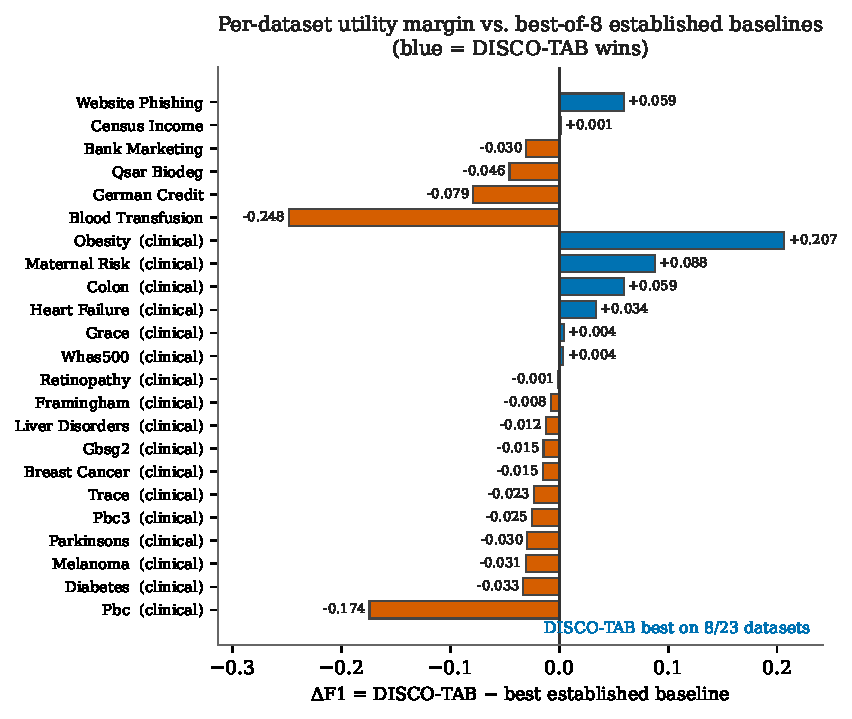
\includegraphics[width=\columnwidth]{fig2_utility_margin.pdf}
\caption{\newexp{Per-dataset utility margin of DISCO-TAB over the best established (GAN/VAE/flow/marginal) baseline ($\Delta F_1$; blue = DISCO-TAB higher). It leads on 9 of 23 datasets, with the largest gains on imbalanced clinical sets.}}
\label{fig:margin}
\end{figure}

\subsection{Minority-Class Recovery and Calibration}
Mean macro-$F_1$ understates what inverse-frequency reward shaping buys, because it is dominated by the majority class. We therefore re-score every generator with three downstream learners (random forest, logistic regression, and gradient-boosted trees) on three further measures: recall of the real minority class, the area under the ROC curve (AUROC), and the area under the precision--recall curve (AUPRC), the more informative summary under heavy imbalance. Table~\ref{tab:downstream_ext} reports the benchmark means. DISCO-TAB recovers the minority class better than any full-coverage competitor, reaching a minority-class recall of $0.61$ against $0.47$ for the next-best generator, and the gap holds under all three classifiers ($0.61$, $0.62$, and $0.59$ for random forest, logistic regression, and XGBoost). On the threshold-free measures it is competitive rather than dominant: its AUROC ($0.76$) is within noise of TAEGAN ($0.75$) and ADS-GAN ($0.74$) and, as Table~\ref{tab:downstream_ext} shows, below both the TRTR reference ($0.80$) and the partial-coverage TabSyn ($0.81$, the best on AUROC and AUPRC alike), so we claim no advantage on these summaries (DISCO-TAB's AUPRC is $0.62$). The decisive signal is the minority-class recall gap: the rare, clinically important class is not merely present in the synthetic data but learnable from it, and because the advantage persists across three different learners it is a property of the data rather than of any single classifier.

\input{downstream_ext_table}

\subsection{Statistical Fidelity}

Utility alone is insufficient, since a generator could score well by memorizing the training data. We therefore ask how faithfully each method reproduces the real distributions, using the Jensen-Shannon divergence (JSD) as the primary measure. For each feature we build its real and synthetic marginal distributions $P$ and $Q$, discretizing continuous features into $20$ equal-width bins over the real feature range; with the mixture $M=\tfrac{1}{2}(P+Q)$,
\begin{equation}
\mathrm{JSD}(P\,\|\,Q) = \tfrac{1}{2}\,D_{KL}(P\,\|\,M) + \tfrac{1}{2}\,D_{KL}(Q\,\|\,M),
\label{eq:jsd}
\end{equation}
where $D_{KL}$ is the Kullback-Leibler divergence; with base-2 logarithms $\mathrm{JSD}\in[0,1]$, smaller is better. For dependency structure we report correlation preservation: one minus the mean absolute difference between off-diagonal entries of the real and synthetic Pearson matrices, so $1$ denotes identical structure. In the utility--fidelity plane (Figure~\ref{fig:tradeoff}), DISCO-TAB sits in the high-utility, low-divergence region alongside RealTabFormer and TAEGAN; its mean JSD ($0.043$) trails the best autoregressive and flow methods, and post-hoc quantile calibration of the numerical columns narrows this gap, making DISCO-TAB the strongest learned full-coverage generator on the KS statistic and the strongest overall on correlation preservation (Table~\ref{tab:aggregate}). The language-based baselines handle discrete columns most naturally, so DISCO-TAB's fidelity edge is sharpest on numeric-heavy clinical data while its categorical handling remains future work. As a sanity check, the independent-marginals baseline behaves exactly as constructed: the lowest marginal divergence of any method (JSD $0.004$, KS $0.028$) yet near the bottom on correlation ($0.82$) and utility, confirming that the marginal-fidelity and dependency metrics capture distinct, non-redundant properties.

\begin{figure}[t]
\centering
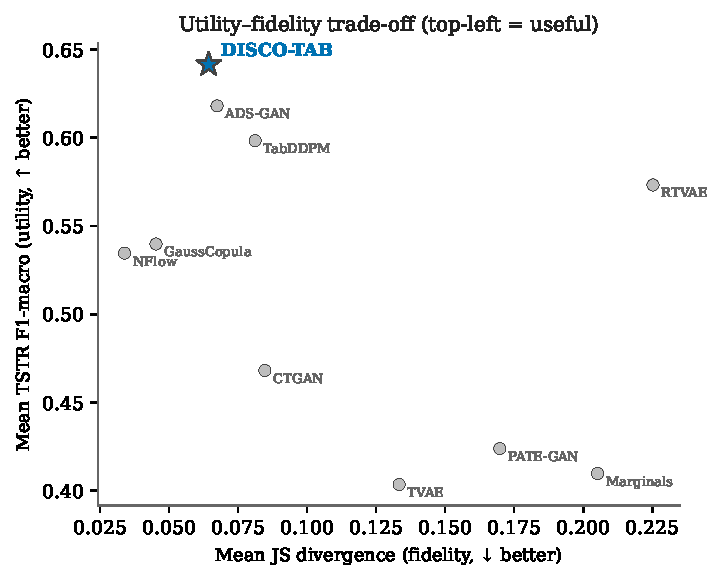
\includegraphics[width=\columnwidth]{fig4_utility_fidelity.pdf}
\caption{\newexp{Utility--fidelity trade-off (top-left best): mean TSTR macro-$F_1$ vs.\ mean Jensen--Shannon divergence. DISCO-TAB combines high utility with low divergence; TabSyn's low divergence comes with collapsed utility.}}
\label{fig:tradeoff}
\end{figure}

\subsection{Empirical Disclosure-Risk Analysis}\label{sec:privacyResults}

A central question is whether generated records reproduce real patients. We measure this with the distance to closest record (DCR), a heuristic proximity indicator rather than a formal guarantee: it does not bound membership-inference (MIA) or attribute-inference attacks. Identically for every method, we one-hot encode categoricals, standardize numerics on the training partition, and take the Euclidean distance to the nearest real neighbor divided by the square root of the encoded dimension. Since DCR depends on encoding, we report each dataset's ratio to a within-dataset real--real baseline (the median nearest-neighbor distance between two disjoint halves of the real test set); a ratio near one means synthetic records are about as far from real records as real records are from each other (Figure~\ref{fig:privacy}(b)).

\begin{figure*}[t]
\centering
\includegraphics[width=0.85\textwidth]{fig_privacy_combined.pdf}
\caption{\newexp{Disclosure risk. (a) Utility vs.\ mean DCR ratio (synthetic over real--real baseline; $1$ = calibrated): DISCO-TAB pairs high utility with a near-calibrated ratio, while TabDDPM inflates it at a cost in utility. (b) Per-dataset DCR ratio: DISCO-TAB stays near the baseline, whereas TabDDPM inflates sharply on small or imbalanced sets (``privacy via noise'').}}
\label{fig:privacy}
\end{figure*}

Across all 23 datasets, DISCO-TAB's DCR ratio stays in a narrow band around one ($\approx\!0.6$--$1.2$), neither copying the data nor drifting from it. TabDDPM is far more erratic, inflating to $6.7\times$ the baseline on Breast Cancer and over $12\times$ on QSAR Biodegradation; such large distances are easily misread as privacy but in fact mark samples pushed off the real manifold, which on small sets coincides with weak utility. DISCO-TAB instead occupies the practical middle ground a governed data-sharing workflow needs. Two training-set checks agree: a DISCO-TAB record is closer to its nearest training record than to its nearest held-out record only $28\%$ of the time ($0.5$ would indicate no bias), below $0.5$ on every dataset, and a distance-based membership test, whether training records lie closer to the synthetic data than held-out records do, gives DISCO-TAB a modest mean AUROC of $0.52$, just above the $0.5$ no-leakage value (third-highest of the fourteen methods, but low in absolute terms; Table~\ref{tab:aggregate}). Its one elevated train-duplicate rate, on the all-categorical Website Phishing set, reflects that set's limited combinatorial support rather than memorization.

Table~\ref{tab:privacy_train} makes the training-set comparison concrete, using the real held-out set as the reference row. Measured against the training data, DISCO-TAB's synthetic records sit slightly farther from the nearest training record than a genuine held-out real sample does and duplicate training rows less often, so on both counts a synthetic DISCO-TAB record discloses no more about the training set than an unseen real patient would. The language-model baselines behave differently: GReaT and RealTabFormer land closer to the training data than the holdout, and RealTabFormer's train-duplicate rate is several times the reference, consistent with partial memorization.

\input{privacy_train_table}

Panel~(a) of Figure~\ref{fig:privacy} summarizes the resulting utility--privacy trade-off across generators: DISCO-TAB pairs high downstream utility with a DCR ratio near one, the regime a governed data-sharing workflow needs; TabDDPM trades utility away for an inflated ratio that signals off-manifold noise rather than genuine protection, while the weakest generators sit at low utility regardless of their distance to the real data.
